	
% This template from http://www.vel.co.nz, originally from http://www.tedpavlic.com

\documentclass{article}
% Change "article" to "report" to get rid of page number on title page
\usepackage{amsmath,amsfonts,amsthm,amssymb, mathrsfs}
\usepackage{bigints}
\usepackage{setspace}
\usepackage{Tabbing}
\usepackage{fancyhdr}
\usepackage{lastpage}
\usepackage{textcomp}
\usepackage{extramarks}
\usepackage{chngpage}
\usepackage{soul,color}
\usepackage{graphicx,float,wrapfig}
\usepackage{cancel}
\usepackage{indentfirst}
\usepackage{mdframed}

% In case you need to adjust margins:
\topmargin=-0.45in      %
\evensidemargin=0in     %
\oddsidemargin=0in      %
\textwidth=6.5in        %
\textheight=9.0in       %
\headsep=0.25in         %

% Homework Specific Information
\newcommand{\hmwkTitle}{WS5}
\newcommand{\hmwkDueDate}{}
\newcommand{\hmwkClass}{Ay\ 190}
\newcommand{\hmwkAuthorName}{Cutter\ Coryell}

% Setup the header and footer
\pagestyle{fancy}                                                       %
\lhead{\hmwkAuthorName}                                                 %
\chead{\hmwkClass\ : \hmwkTitle}  %
\rhead{\hmwkDueDate}                                                     %
\renewcommand\headrulewidth{0.4pt}                                      %
\renewcommand\footrulewidth{0.4pt}                                      %

% This is used to trace down (pin point) problems
% in latexing a document:
%\tracingall

%%%%%%%%%%%%%%%%%%%%%%%%%%%%%%%%%%%%%%%%%%%%%%%%%%%%%%%%%%%%%
% Some tools
\newcommand{\enterProblemHeader}[1]{\nobreak\extramarks{#1}{#1 continued on next page\ldots}\nobreak%
                                    \nobreak\extramarks{#1 (continued)}{#1 continued on next page\ldots}\nobreak}%
\newcommand{\exitProblemHeader}[1]{\nobreak\extramarks{#1 (continued)}{#1 continued on next page\ldots}\nobreak%
                                   \nobreak\extramarks{#1}{}\nobreak}%

\newlength{\labelLength}
\newcommand{\labelAnswer}[2]
  {\settowidth{\labelLength}{#1}%
   \addtolength{\labelLength}{0.25in}%
   \changetext{}{-\labelLength}{}{}{}%
   \noindent\fbox{\begin{minipage}[c]{\columnwidth}#2\end{minipage}}%
   \marginpar{\fbox{#1}}%

   % We put the blank space above in order to make sure this
   % \marginpar gets correctly placed.
   \changetext{}{+\labelLength}{}{}{}}%

\setcounter{secnumdepth}{0}
\newcommand{\homeworkProblemName}{}%
\newcounter{homeworkProblemCounter}%
\newenvironment{homeworkProblem}[1][Problem \arabic{homeworkProblemCounter}]%
  {\stepcounter{homeworkProblemCounter}%
   \renewcommand{\homeworkProblemName}{#1}%
   \section{\homeworkProblemName}%
   \enterProblemHeader{\homeworkProblemName}}%
  {\exitProblemHeader{\homeworkProblemName}}%

\newcommand{\problemAnswer}[1]
  {\noindent\fbox{\begin{minipage}[c]{\columnwidth}#1\end{minipage}}}%

\newcommand{\problemLAnswer}[1]
  {\labelAnswer{\homeworkProblemName}{#1}}

\newcommand{\homeworkSectionName}{}%
\newlength{\homeworkSectionLabelLength}{}%
\newenvironment{homeworkSection}[1]%
  {% We put this space here to make sure we're not connected to the above.
   % Otherwise the changetext can do funny things to the other margin

   \renewcommand{\homeworkSectionName}{#1}%
   \settowidth{\homeworkSectionLabelLength}{\homeworkSectionName}%
   \addtolength{\homeworkSectionLabelLength}{0.25in}%
   \changetext{}{-\homeworkSectionLabelLength}{}{}{}%
   \subsection{\homeworkSectionName}%
   \enterProblemHeader{\homeworkProblemName\ [\homeworkSectionName]}}%
  {\enterProblemHeader{\homeworkProblemName}%

   % We put the blank space above in order to make sure this margin
   % change doesn't happen too soon (otherwise \sectionAnswer's can
   % get ugly about their \marginpar placement.
   \changetext{}{+\homeworkSectionLabelLength}{}{}{}}%

\newcommand{\sectionAnswer}[1]
  {% We put this space here to make sure we're disconnected from the previous
   % passage

   \noindent\fbox{\begin{minipage}[c]{\columnwidth}#1\end{minipage}}%
   \enterProblemHeader{\homeworkProblemName}\exitProblemHeader{\homeworkProblemName}%
   \marginpar{\fbox{\homeworkSectionName}}%

   % We put the blank space above in order to make sure this
   % \marginpar gets correctly placed.
   }%

\newenvironment{myindentpar}[1]%
 {\begin{list}{}%
         {\setlength{\leftmargin}{#1}}%
         \item[]%
 }
 {\end{list}}

%%%%%%%%%%%%%%%%%%%%%%%%%%%%%%%%%%%%%%%%%%%%%%%%%%%%%%%%%%%%%


%%%%%%%%%%%%%%%%%%%%%%%%%%%%%%%%%%%%%%%%%%%%%%%%%%%%%%%%%%%%%
% Make title
\title{\vspace{2in}\textmd{\textbf{\hmwkClass:\ \hmwkTitle}}\\\normalsize\vspace{0.1in}\small{Due\ on\ \hmwkDueDate}\\\vspace{0.1in}\large{\textit{\hmwkClassInstructor\ \hmwkClassTime}}\vspace{3in}}
\date{}
\author{\textbf{\hmwkAuthorName}}
%%%%%%%%%%%%%%%%%%%%%%%%%%%%%%%%%%%%%%%%%%%%%%%%%%%%%%%%%%%%%

%%%% MY COMMANDS %%%%%%%%%%%%%%%%%%%%%

\newcommand{\deri}[2]{\frac{\mathrm{d} #1}{\mathrm{d} #2}}
\newcommand{\pderi}[2]{\frac{\partial #1}{\partial #2}}
\newcommand{\inte}[4]{\int_{#1}^{#2} \! #3 \, \mathrm{d} #4}
\newcommand{\ointe}[4]{\oint_{#1}^{#2} \! #3 \, \mathrm{d} #4}
\newcommand{\del}{\nabla}
\newcommand{\D}{\mathrm{d}}
\newcommand{\ee}[1]{\times 10^{#1}}
\newcommand{\fpe}{\frac{1}{4 \pi \epsilon_0}}
\newcommand{\bra}[1]{\left< #1 \right|}
\newcommand{\ket}[1]{\left| #1 \right>}
\newcommand{\cket}[1]{\left. #1 \right>}


% Distance units
\newcommand{\m}[0]{\text{\ m}}
\newcommand{\cm}[0]{\text{\ cm}}
\newcommand{\km}[0]{\text{\ km}}
\newcommand{\pc}[0]{\text{\ pc}}
\newcommand{\kpc}[0]{\text{\ kpc}}
\newcommand{\Mpc}[0]{\text{\ Mpc}}
\newcommand{\Gpc}[0]{\text{\ Gpc}}
\newcommand{\lyr}[0]{\text{\ lyr}}
\newcommand{\Rs}[0]{R_\odot}

% Mass units
\newcommand{\g}[0]{\text{\ g}}
\newcommand{\kg}[0]{\text{\ kg}}
\newcommand{\Ms}[0]{M_\odot}

% Time units
\newcommand{\s}[0]{\text{\ s}}
\newcommand{\days}[0]{\text{\ days}}
\newcommand{\yr}[0]{\text{\ yr}}
\newcommand{\Hz}[0]{\text{\ Hz}}
\newcommand{\kHz}[0]{\text{\ kHz}}
\newcommand{\MHz}[0]{\text{\ MHz}}
\newcommand{\GHz}[0]{\text{\ GHz}}
\newcommand{\THz}[0]{\text{\ THz}}

% Energy units
\newcommand{\erg}[0]{\text{\ erg}}
\newcommand{\J}[0]{\text{\ J}}
\newcommand{\eV}[0]{\text{\ eV}}
\newcommand{\meV}[0]{\text{\ meV}}
\newcommand{\keV}[0]{\text{\ keV}}
\newcommand{\MeV}[0]{\text{\ MeV}}
\newcommand{\GeV}[0]{\text{\ GeV}}
\newcommand{\TeV}[0]{\text{\ TeV}}

% Force units
\newcommand{\N}[0]{\text{\ N}}
\newcommand{\dyn}[0]{\text{\ dyn}}

% Power units
\newcommand{\W}[0]{\text{\ W}}
\newcommand{\Ls}[0]{L_\odot}

% Temperature units
\newcommand{\K}[0]{\text{\ K}}
\newcommand{\degC}[0]{\text{\ \(^\circ\)C}}
\newcommand{\degF}[0]{\text{\ \(^\circ\)F}}

% Electromagnetic units
\newcommand{\V}[0]{\text{\ V}}
\newcommand{\kV}[0]{\text{\ kV}}
\newcommand{\C}[0]{\text{\ C}}
\newcommand{\esu}[0]{\text{\ esu}}
\newcommand{\T}[0]{\text{\ T}}
\newcommand{\G}[0]{\text{\ G}}


\newcount\colveccount
\newcommand*\colvec[1]{
        \global\colveccount#1
        \begin{pmatrix}
        \colvecnext
}
\def\colvecnext#1{
        #1
        \global\advance\colveccount-1
        \ifnum\colveccount>0
                \\
                \expandafter\colvecnext
        \else
                \end{pmatrix}
        \fi
}

%%%%%%%%%%%%%%%%%%%%%%%%%%%%%%%%%%

\begin{document}
\begin{spacing}{1.1}

\newpage

% When problems are long, it may be desirable to put a \newpage or a
% \clearpage before each homeworkProblem environment

I worked with no one on this worksheet. It took about \(3\ee{14}\) cm to complete (3 hours).

\subsection{Curve Fitting}

\noindent (a)

First I plotted the raw data, without any fitting.

\begin{figure}[H]
\begin{centering}
 \hspace{-1cm} 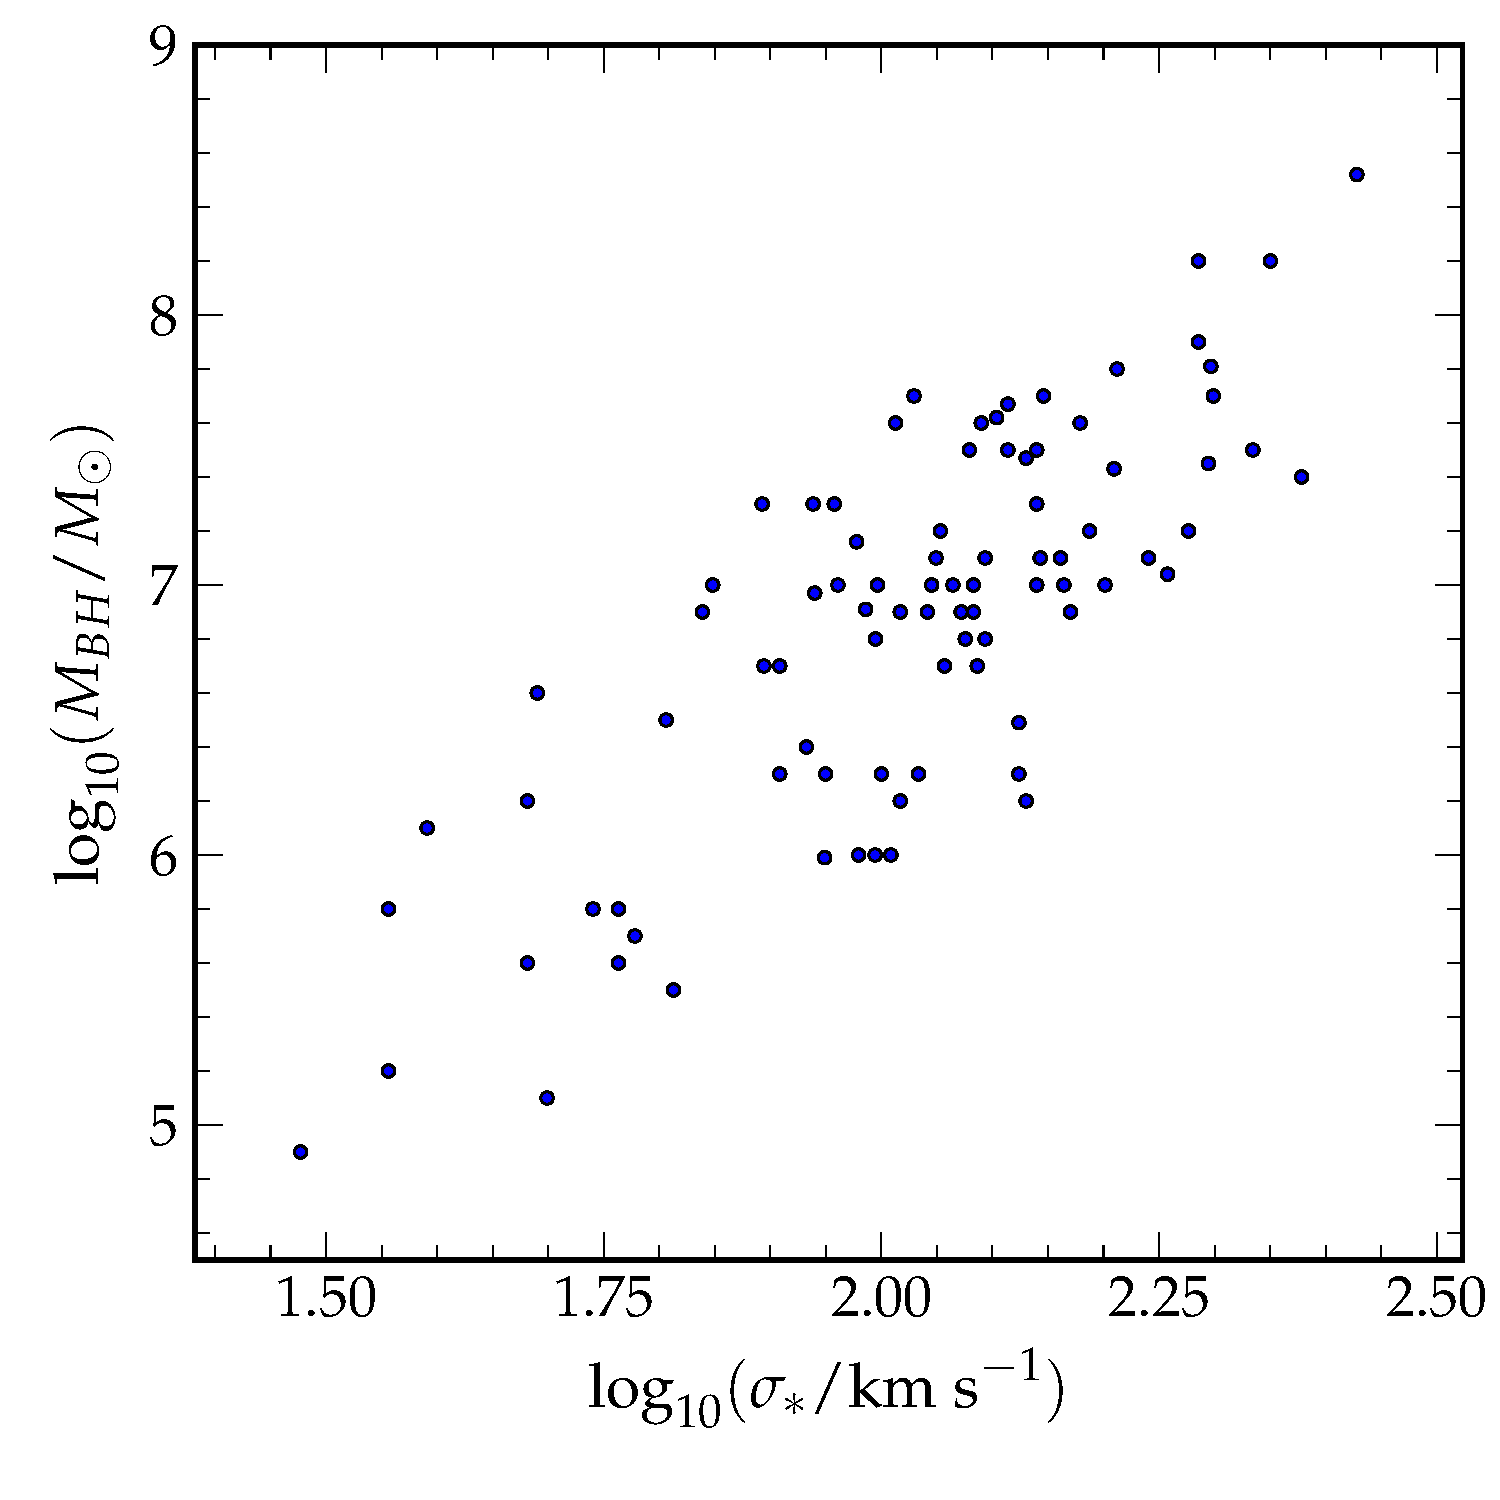
\includegraphics[width=0.8\textwidth]{part-a.pdf}
 \caption{The relation between stellar velocity disperson \(\sigma_*\) in a galaxy bulge and the mass \(M_{\sc BH}\) of the supermassive black hole at the center of the galaxy.}
 \label{fig-a}
\end{centering}
\end{figure} 

\newpage

\noindent (b)

Then I fit the data to a linear function, ignoring the errors in \(M_{\sc BH}\). I did this by setting all the \(\sigma_i\) to a constant (specifically, 1 -- the exactly constant value doesn't matter, because it ultimately cancels in the definitions of \(a_1\) and \(a_2\)).

\begin{figure}[H]
\begin{centering}
 \hspace{-1cm} 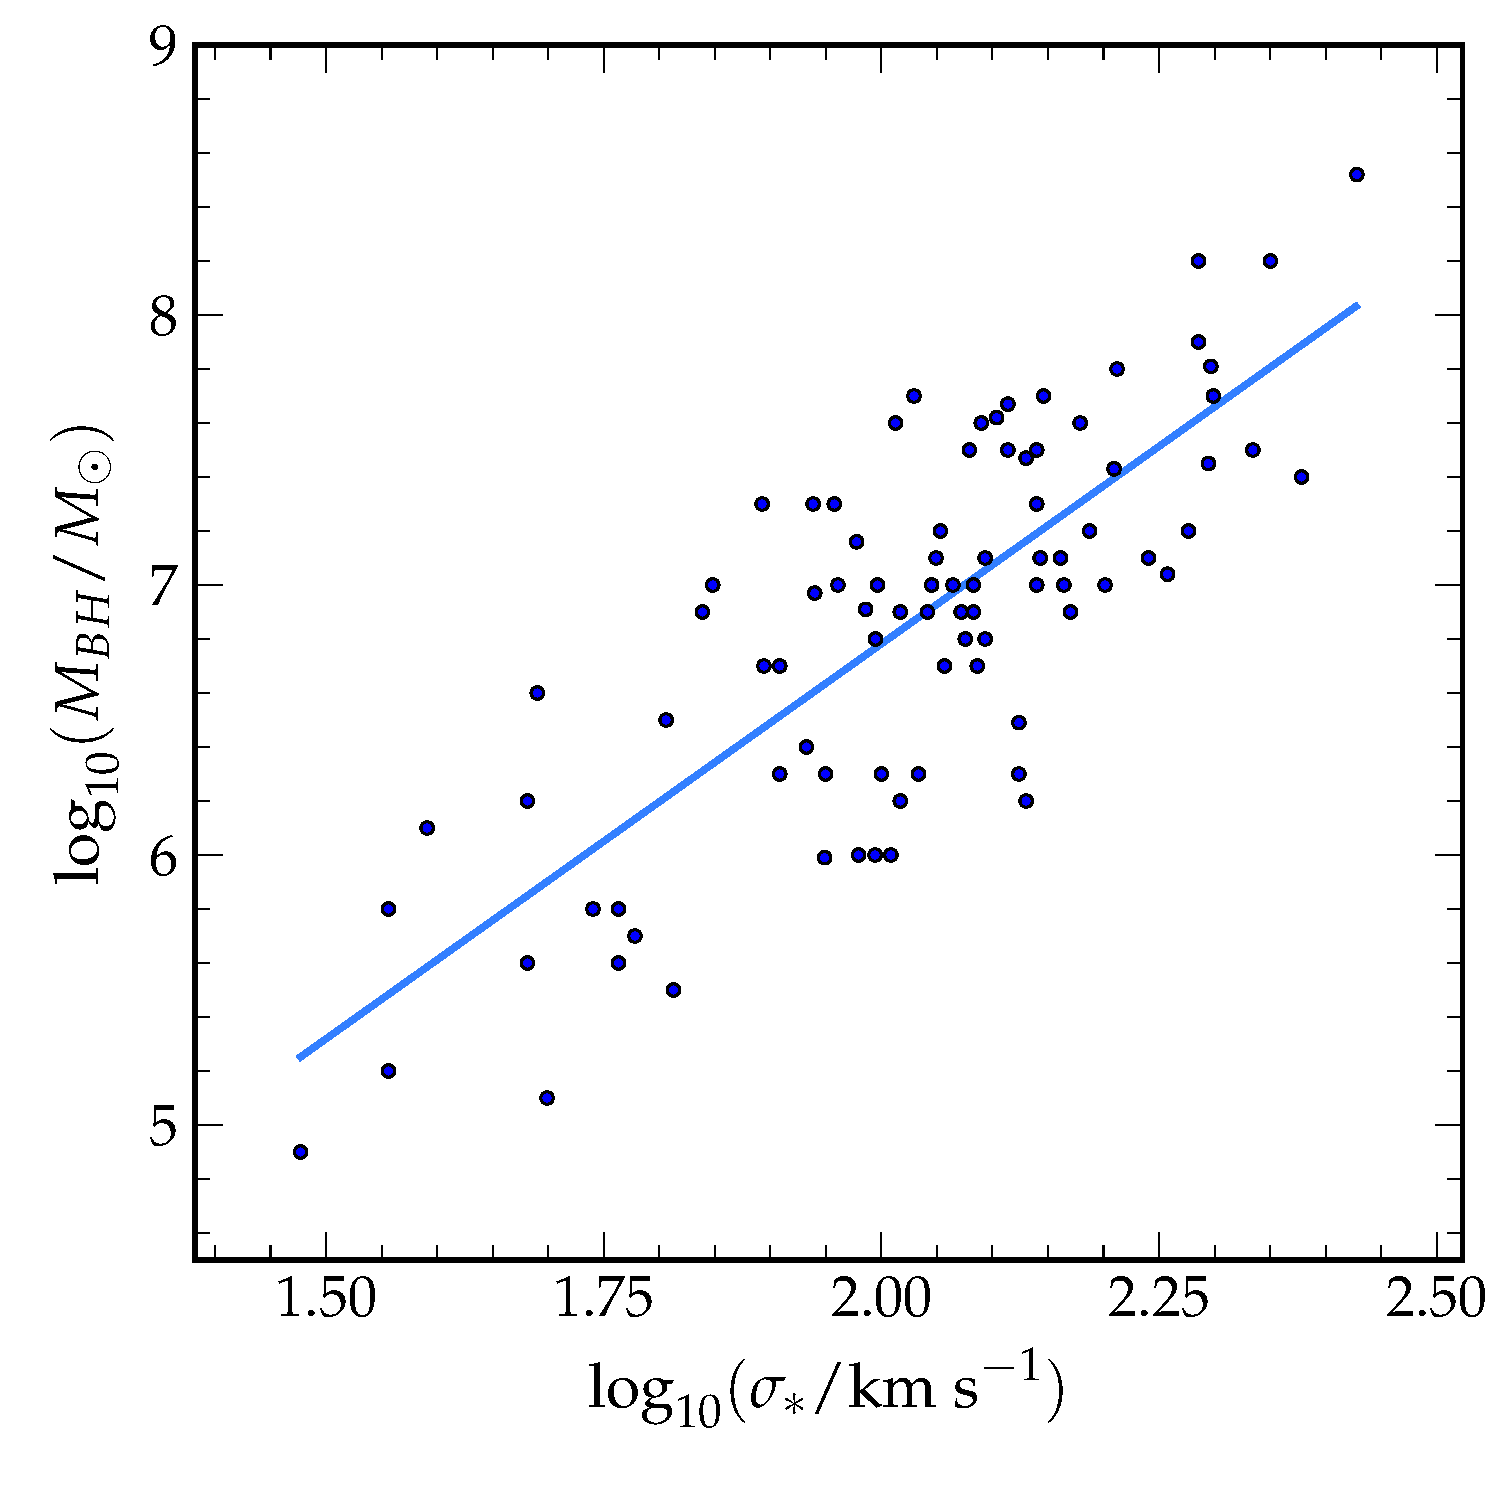
\includegraphics[width=0.8\textwidth]{part-b.pdf}
 \caption{The relation between stellar velocity disperson \(\sigma_*\) in a galaxy bulge and the mass \(M_{\sc BH}\) of the supermassive black hole at the center of the galaxy. A linear fit of the data, ignoring errors, is given.}
 \label{fig-b}
\end{centering}
\end{figure} 

\newpage

I then rescaled my plot and overlaid its data points with those of Greene \& Ho so that the linear fits could be compared. Clearly there is a somewhat large discrepancy between the fits, with a \(9^\circ\) angle between the two fit lines. Because this angle is dependent on the x-y plot scaling, it is meaningless by itself, but I will soon use it to assess how much closer to Greene \& Ho's fit my next fit will be. I can think of two reasons for this discrepancy: first, Greene \& Ho have data that I lack, almost all of which is above my line on the right side of the plot, which helps to explains why mine dips lower than theirs toward the right. Secondly, their fit undoubtedly takes error into account, which may help to further explain the discrepancy.

\begin{figure}[H]
\begin{centering}
 \hspace{-1cm} 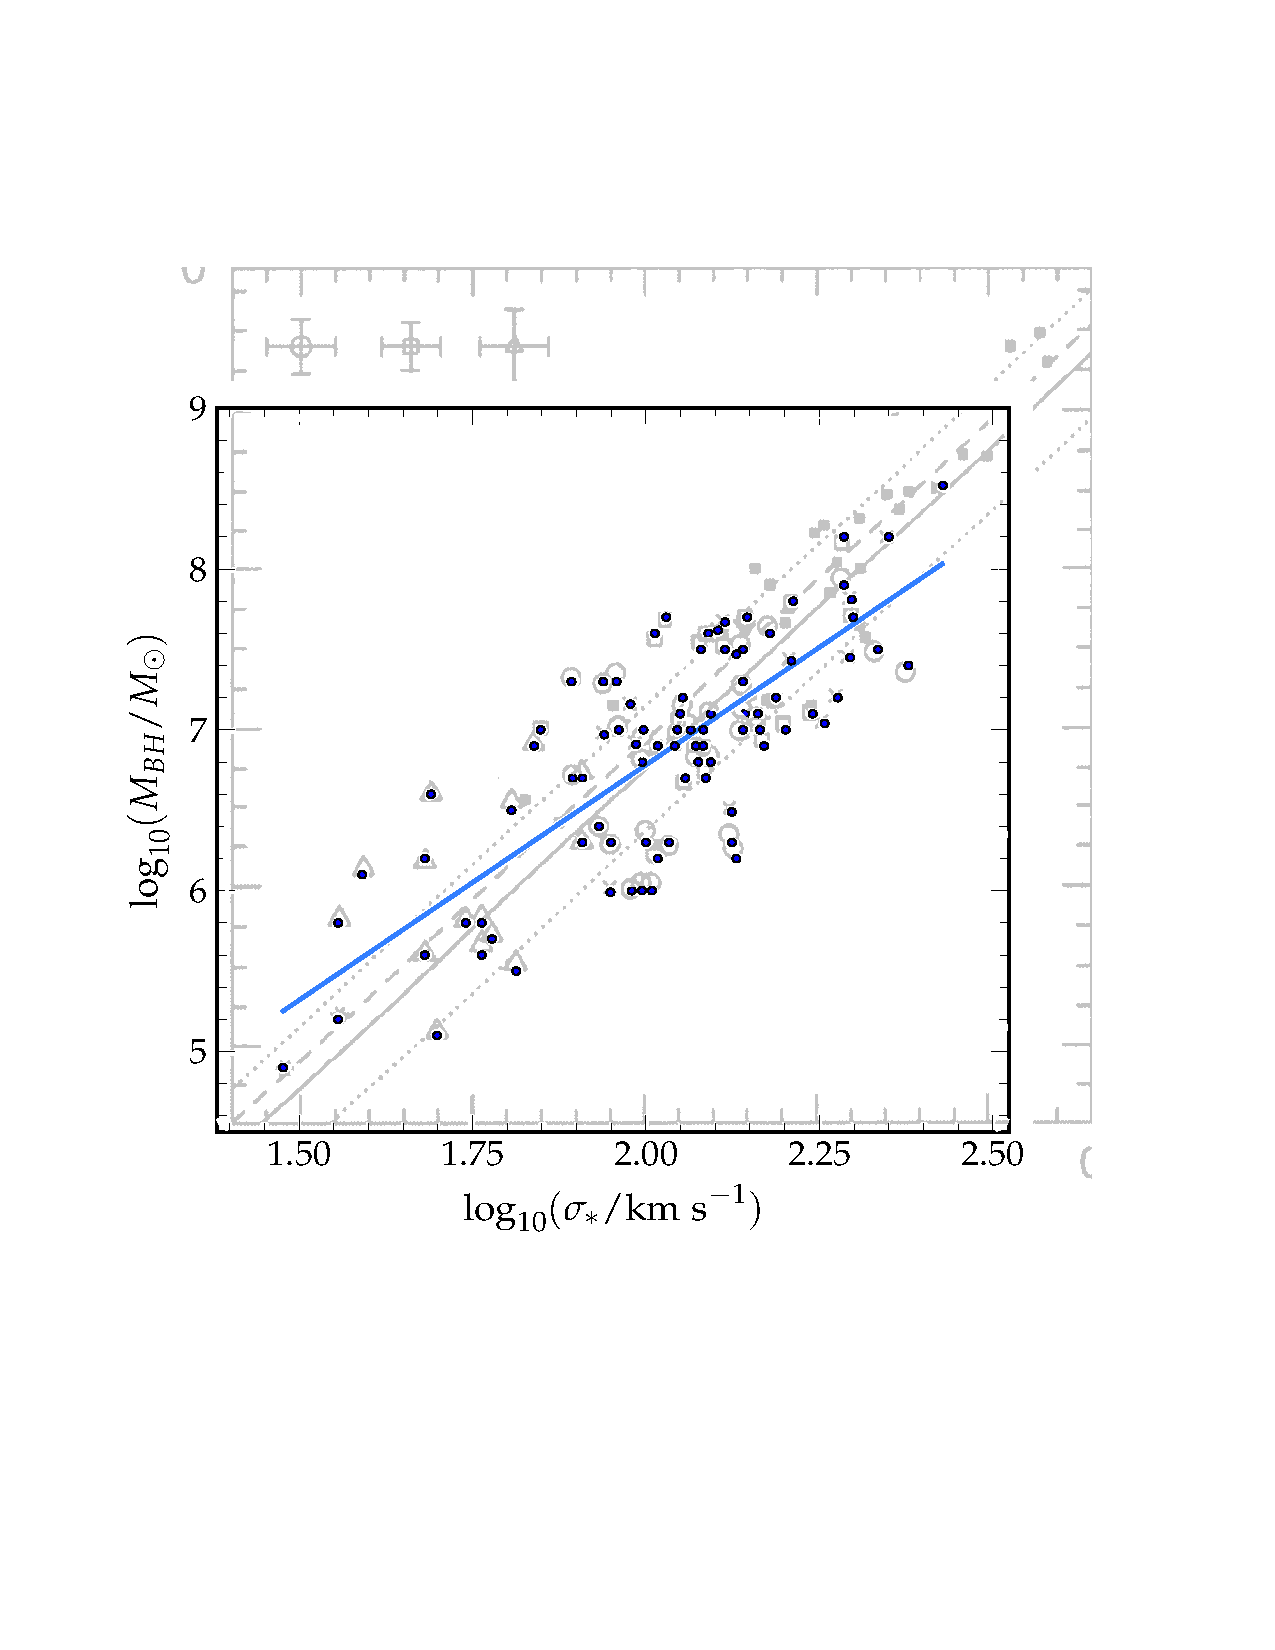
\includegraphics[width=0.8\textwidth]{overlay.pdf}
 \caption{The relation between stellar velocity disperson \(\sigma_*\) in a galaxy bulge and the mass \(M_{\sc BH}\) of the supermassive black hole at the center of the galaxy. Our plot and linear fit is superimposed with the plot and linear fit of Greene \& Ho.}
 \label{fig-overlay}
\end{centering}
\end{figure} 

\newpage

\noindent (c)

I then fit the data including errors in ; the result is the red dashed line in Fig.~\ref{fig-c}. I chose to use the error titled ``Formal uncertainty (or lower limit) in logM'' because it was the only one of the two error columns for logM that contained an error for each logM value.

\begin{figure}[H]
\begin{centering}
 \hspace{-1cm} 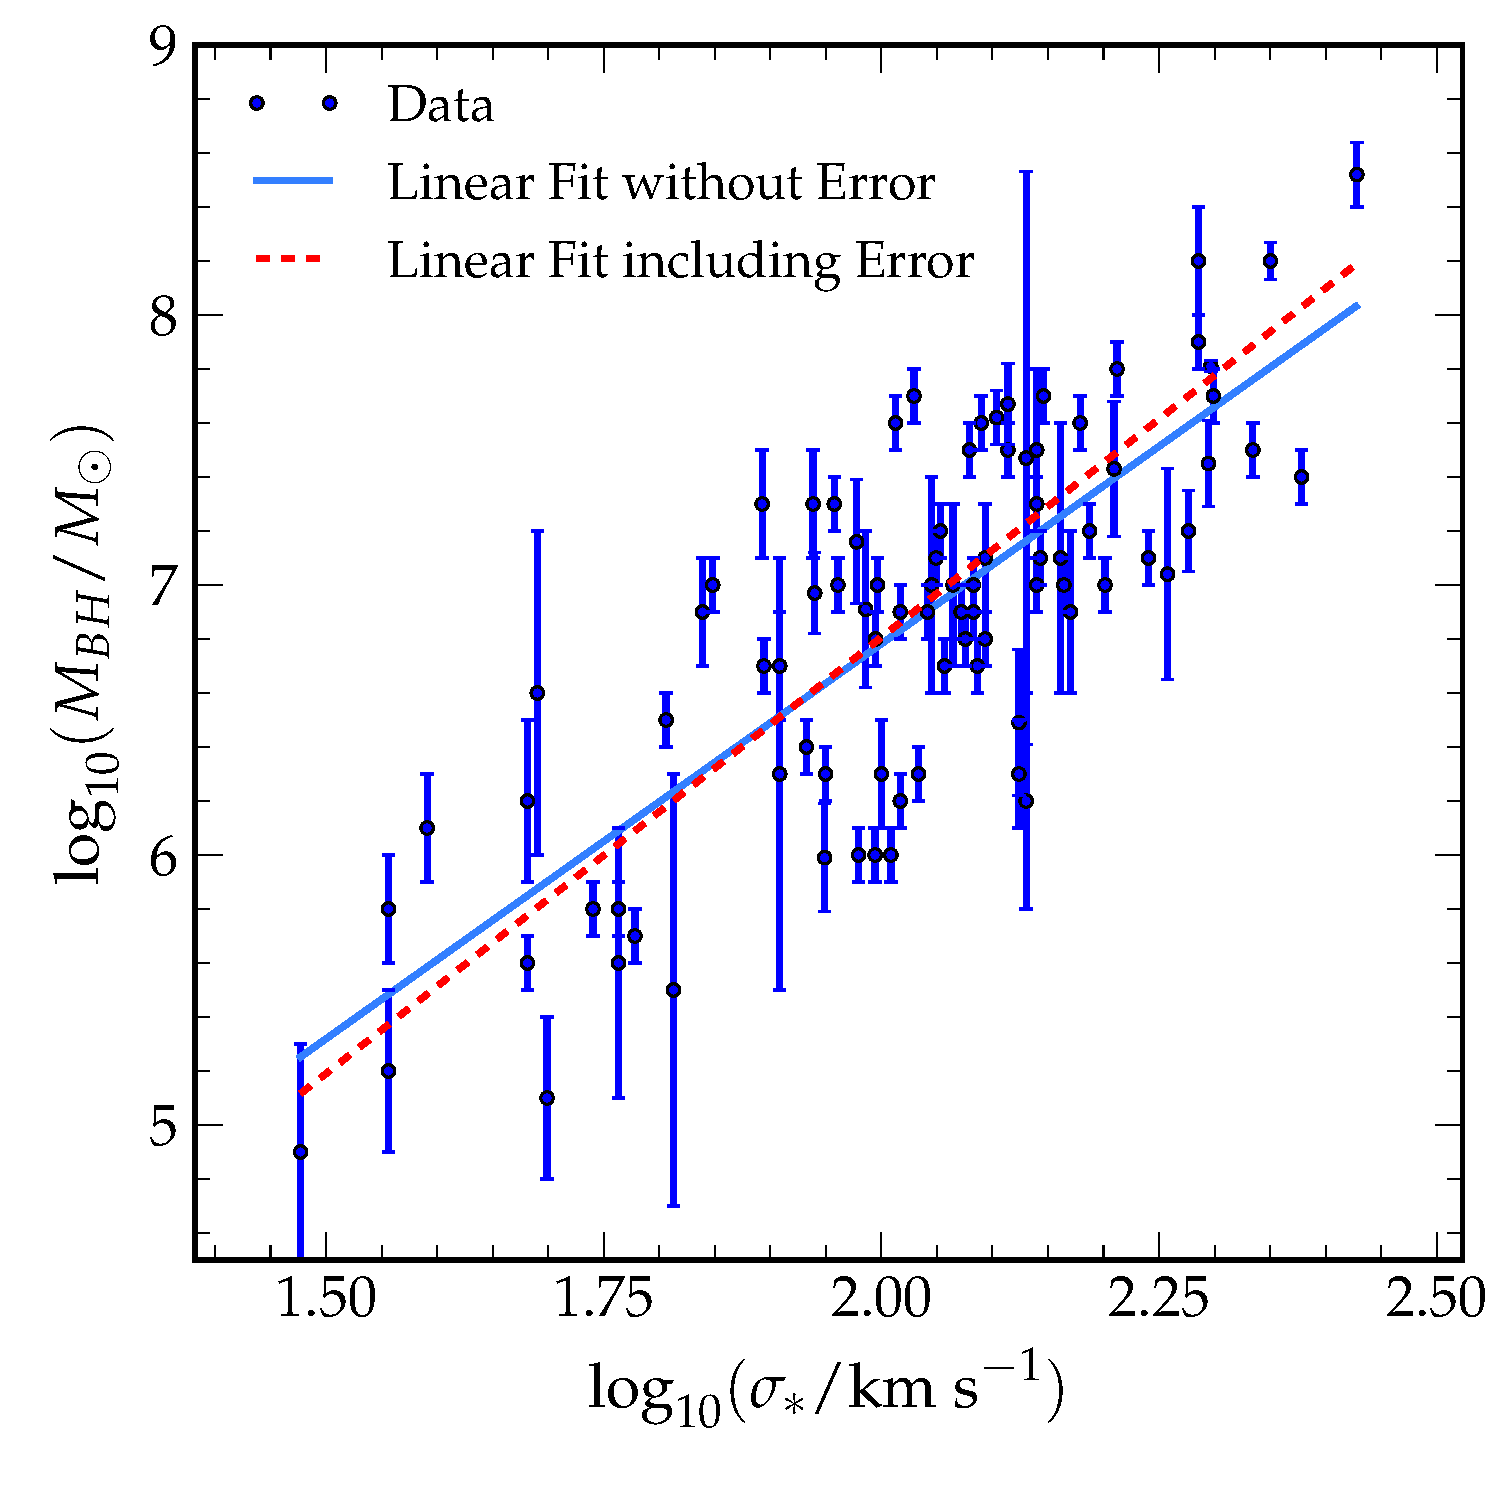
\includegraphics[width=0.8\textwidth]{part-c.pdf}
 \caption{The relation between stellar velocity disperson \(\sigma_*\) in a galaxy bulge and the mass \(M_{\sc BH}\) of the supermassive black hole at the center of the galaxy. Two linear fits of the data, one ignoring errors (blue) and one including errors (red), are given.}
 \label{fig-c}
\end{centering}
\end{figure} 

This inclusion of errors in \(M_{\sc BH}\) results in a linear fit closer to that of Greene \& Ho. The discrepancy in angle between the fits has been reduced from \(9^\circ\) to \(5^\circ\), a reduction in the discrepancy of 44\%.

\end{spacing}
\end{document}

%%%%%%%%%%%%%%%%%%%%%%%%%%%%%%%%%%%%%%%%%%%%%%%%%%%%%%%%%%%%%
